% $Header: /cvsroot/latex-beamer/latex-beamer/solutions/conference-talks/conference-ornate-20min.en.tex,v 1.6 2004/10/07 20:53:08 tantau Exp $

\documentclass[trans,aspectratio=1610]{beamer}
\usepackage{etex}
\newcommand\orh{\mbox{ ; }}
% This file is a solution template for:
\usepackage{amsmath}
\usepackage{amsthm,amssymb,mathabx,amsbsy}
\usepackage{xspace}
\usepackage[all]{xy}
% - Talk at a conference/colloquium.
% - Talk length is about 20min.
% - Style is ornate.
\DeclareMathOperator*{\argmax}{arg\,max}
\DeclareMathOperator*{\argmin}{arg\,min}
\newcommand{\defprog}{\ensuremath{P}\xspace}
\newcommand{\lpnot}[1][\!\!]{\sim#1}
\newcommand{\defpprog}{\ensuremath{\mathcal{P}}\xspace}
\newcommand{\lpif}{\leftarrow}

% Copyright 2004 by Till Tantau <tantau@users.sourceforge.net>.
%
% In principle, this file can be redistributed and/or modified under
% the terms of the GNU Public License, version 2.
%
% However, this file is supposed to be a template to be modified
% for your own needs. For this reason, if you use this file as a
% template and not specifically distribute it as part of a another
% package/program, I grant the extra permission to freely copy and
% modify this file as you see fit and even to delete this copyright
% notice.
%\usepackage{xcolor}
\usepackage{graphicx}
\usepackage{array}
\usepackage[all]{xy}
%\usepackage{theapa}
\usepackage{tikz}
\usetikzlibrary{snakes,arrows,shapes,arrows.meta}

\usetikzlibrary{shapes.geometric}
\usetikzlibrary{shadows}
\usetikzlibrary{positioning}
\usepackage{algorithm}
%\usepackage{algorithmic}
\usepackage{algpseudocode}
\usepackage{natbib}

\usepackage{apalike}
\mode<presentation>
{
%  \usetheme{AnnArbor}
%  \usetheme{Antibes}
%  \usetheme{Bergen}
%  \usetheme{Berkeley}
%  \usetheme{Berlin}
%  \usetheme{Boadilla}
%  \usetheme{boxes}
%  \usetheme{CambridgeUS}
%  \usetheme{Copenhagen}
%  \usetheme{Darmstadt}
%  \usetheme{default}
%  \usetheme{Dresden}
%  \usetheme{Frankfurt}
%  \usetheme{Goettingen}
%  \usetheme{Hannover}
%  \usetheme{Ilmenau}
%  \usetheme{JuanLesPins}
%  \usetheme{Luebeck}
%  \usetheme{Madrid}
%  \usetheme{Malmoe}
%  \usetheme{Marburg}
%  \usetheme{Montpellier}
%  \usetheme{PaloAlto}
%  \usetheme{Pittsburgh}
%  \usetheme{Rochester}
%  \usetheme{Singapore}
%  \usetheme{Szeged}
%  \usetheme{Warsaw}
  \usetheme{PLP}

%\usecolortheme{lily}%
  % or ...

  \setbeamercovered{transparent}
  % or whatever (possibly just delete it)
}

\newcommand\cA{{\cal A}}
\newcommand\cB{{\cal B}}
\newcommand\cC{{\cal C}}
\newcommand\cD{{\cal D}}
\newcommand\cE{{\cal E}}
\newcommand\cF{{\cal F}}
\newcommand\cG{{\cal G}}
\newcommand\cH{{\cal H}}
\newcommand\cI{{\cal I}}
\newcommand\cJ{{\cal J}}
\newcommand\cK{{\cal K}}
\newcommand\cL{{\cal L}}
\newcommand\cN{{\cal N}}
\newcommand\cP{{\cal P}}
\newcommand\cR{{\cal R}}
\newcommand\cS{{\cal S}}
\newcommand\cT{{\cal T}}
\newcommand\cU{{\cal U}}
\newcommand\cV{{\cal V}}
\newcommand\cW{{\cal W}}
\newcommand\cX{{\cal X}}
\newcommand\cM{{\cal M}}
\newcommand\f{\litF}
\newcommand\WMC{\mathit{WMC}}
\newcommand{\pair}[2]{\ensuremath{\langle {#1}, {#2}\rangle}}
\newcommand{\vecranvar}[1]{%
\ensuremath{\mathbf{\ranvar{#1}}}}
\newcommand{\ranvar}[1]{%
\ensuremath{{#1}}}
\newcommand{\fp}{\mathit{fp}}
\newcommand{\tp}{\mathit{tp}}
\newcommand{\TP}{\mathit{TP}}
\newcommand{\FP}{\mathit{FP}}
\newcommand{\TN}{\mathit{TN}}
\newcommand{\FN}{\mathit{FN}}



\usepackage[english]{babel}
% or whatever

%\usepackage[latin1]{inputenc}
% or whatever

\usepackage{times}
\usepackage[T1]{fontenc}
% Or whatever. Note that the encoding and the font should match. If T1
% does not look nice, try deleting the line with the fontenc.
\newcommand{\myalert}[1]{{%\color{red}
 #1}}
\newcommand{\fluffy}{\mathit{fluffy}}
\newcommand{\bdd}[2]
{
\begin{center}
\begin{tikzpicture}
[every node/.style={font=\scriptsize,minimum height=0.5cm,minimum width=0.5cm},x=2cm,y=1.2cm,rounded corners=2mm,zeroarrow/.style = {-stealth,dashed},
  onearrow/.style = {-stealth,solid},
  c/.style = {circle,draw,solid,minimum width=2em,
        minimum height=2em},
  r/.style = {rectangle,draw,solid,minimum width=2em,
        minimum height=2em}]
%[place/.style={shape=ellipse}]
%,draw=blue!50,fill=blue!20,thick,inner sep=0pt,minimum size=6mm},

\node[c] (X11) at (0,1) {#1};
   \node[c] (X21) at (1,1.5) {#2};
   \node[r] (final-one) at (2,0.5) {1};
   \node[r] (final-zero) at (2,1.5){0};
\node[] (lX11) at (0,0) {#1};
   \node (lX21) at (1,0) {#2};


   \path[onearrow,bend right=20] (X11) edge (final-one) ;
   \path[onearrow,bend right=20] (X21) edge   (final-one) ;

%      \draw[onearrow] (X11) -- (final-one);
%   \draw[onearrow] (X21) -- (final-one);

   \path[zeroarrow,bend left=20] (X11) edge  (X21) ;
   \path[zeroarrow,bend left=20] (X21) edge  (final-zero) ;
%
%   \draw[zeroarrow] (X11) -- (X21);
%   \draw[zeroarrow] (X21) -- (final-zero);
%
%\node (root) at ( 0,1) {};
%\node (node21) at ( 1,1.5){}  ;
%\node (0) at ( 2,1.5) {0};
%\node (1) at ( 2,0.5) {1};
%\path[-,bend left](node21) edge (0) (root) edge node {0} (node21);
%\path[-,bend right]
%			 (root) edge (1)
%(node21) edge (1);
\end{tikzpicture}
\end{center}
}


\newcommand{\mdd}
{
\begin{center}
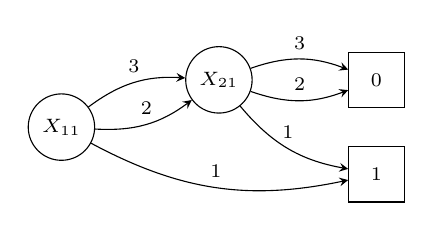
\begin{tikzpicture}
[every node/.style={font=\scriptsize},x=2cm,y=1.2cm,
zeroarrow/.style = {-stealth,dashed},
  onearrow/.style = {-stealth,solid},
  c/.style = {circle,draw,solid,minimum width=2em,
        minimum height=2em},
  r/.style = {rectangle,draw,solid,minimum width=2em,
        minimum height=2em}]
%[place/.style={shape=ellipse}]
%,draw=blue!50,fill=blue!20,thick,inner sep=0pt,minimum size=6mm},

\node[c] (X11) at (0,1) {$X_{11}$};
   \node[c] (X21) at (1,1.5) {$X_{21}$};
   \node[r] (final-one) at (2,0.5) {1};
   \node[r] (final-zero) at (2,1.5){0};

   \path[onearrow,bend right=20] (X11) edge   node [above,midway] {1}(final-one) ;
   \path[onearrow,bend right=20] (X21) edge   node [above,midway] {1}(final-one) ;

   \path[onearrow,bend right=20] (X11) edge   node [above,midway] {2}(X21) ;
   \path[onearrow,bend left=20] (X11) edge   node [above,midway] {3}(X21) ;
   \path[onearrow,bend right=20] (X21) edge   node [above,midway] {2}(final-zero) ;
   \path[onearrow,bend left=20] (X21) edge   node [above,midway] {3}(final-zero) ;
%
%\node (root) at ( 0,1) {};
%\node (node21) at ( 1,1.5){}  ;
%\node (0) at ( 2,1.5) {0};
%\node (1) at ( 2,0.5) {1};
%\path[-,bend left](node21) edge (0) (root) edge node {0} (node21);
%\path[-,bend right]
%			 (root) edge (1)
%(node21) edge (1);
\end{tikzpicture}
\end{center}
}
\newcommand{\mn}{
\begin{center}
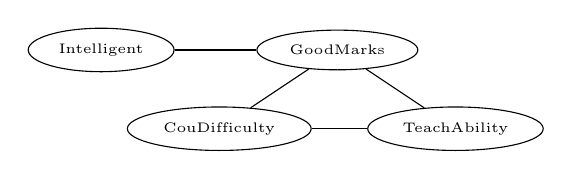
\begin{tikzpicture}
[every node/.style={ellipse,draw,font=\tiny},x=1.5cm,y=1cm]
%[place/.style={shape=ellipse}]
%,draw=blue!50,fill=blue!20,thick,inner sep=0pt,minimum size=6mm},
\node (VisitToAsia) at ( 0,1) {Intelligent};
\node (Tubercolosis) at ( 2,1) [ellipse,draw] {GoodMarks};
\node (Asthma) at ( 1,0) [ellipse,draw] {CouDifficulty};
\node (Cough) at ( 3,0) [ellipse,draw] {TeachAbility};
\path (VisitToAsia) edge  (Tubercolosis)
			 (Tubercolosis) edge (Asthma) edge (Cough)
			(Asthma) edge (Cough);
\end{tikzpicture}\end{center}}

\newcommand{\mln}{
\begin{center}
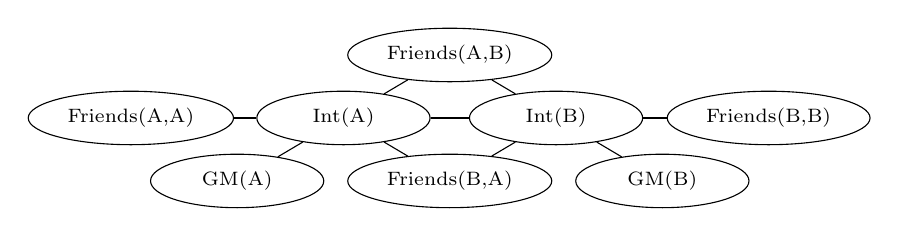
\begin{tikzpicture}
%[every node/.style={ellipse,draw,font=\scriptsize,minimum height=0.5cm,minimum width=2.5cm,
[every node/.style={ellipse,draw,font=\scriptsize,minimum width=2.2cm},x=2.7cm,y=0.8cm]

%[place/.style={shape=ellipse}]
%,draw=blue!50,fill=blue!20,thick,inner sep=0pt,minimum size=6mm},
\node (FriendsAB) at ( 1.5,2) {Friends(A,B)};
\node (FriendsAA) at ( 0,1)  {Friends(A,A)};
\node (FriendsBB) at ( 3,1)  {Friends(B,B)};
\node (FriendsBA) at ( 1.5,0)  {Friends(B,A)};
\node (SmokesA) at ( 1,1)  {Int(A)};
\node (SmokesB) at ( 2,1)  {Int(B)};
\node (CancerA) at ( 0.5,0)  {GM(A)};
\node (CancerB) at ( 2.5,0)  {GM(B)};
\path (FriendsAA) edge  (SmokesA)
		(CancerA) edge (SmokesA)
	(FriendsBB) edge  (SmokesB)
		(CancerB) edge (SmokesB)
	(FriendsAB) edge  (SmokesA)
					edge  (SmokesB)
	(FriendsBA) edge  (SmokesA)
					edge  (SmokesB)
			(SmokesB) edge (SmokesA);

%			 (Tubercolosis) edge (Asthma) edge (Cough)
%			(Asthma) edge (Cough);
\end{tikzpicture}
\end{center}
}


\newcommand{\bn}{
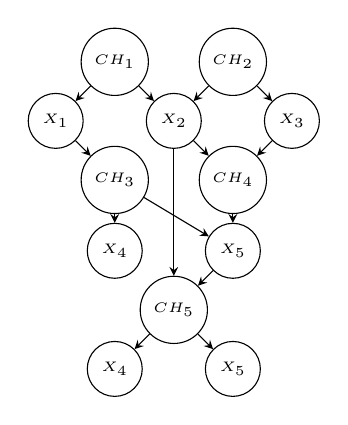
\begin{tikzpicture}
[every node/.style={draw,font=\tiny},x=0.75cm,y=0.75cm,rounded corners=2mm,zeroarrow/.style = {-stealth,dashed},
  onearrow/.style = {-stealth,solid},
  c/.style = {circle,draw,solid},
  r/.style = {rectangle,draw,solid,minimum width=1em,
        minimum height=1em}]
%[place/.style={shape=ellipse}]
%,draw=blue!50,fill=blue!20,thick,inner sep=0pt,minimum size=6mm},

\node[c] (CH1) at (1,5) {$CH_1$};
\node[c] (CH2) at (3,5) {$CH_2$};
\node[c] (X1) at (0,4) {$X_1$};
\node[c] (X2) at (2,4) {$X_2$};
\node[c] (X3) at (4,4) {$X_3$};
\node[c] (CH3) at (1,3) {$CH_3$};
\node[c] (CH4) at (3,3) {$CH_4$};
\node[c] (X4) at (1,1.8) {$X_4$};
\node[c] (X5) at (3,1.8) {$X_5$};
\node[c] (CH5) at (2,0.8) {$CH_5$};
\node[c] (X6) at (1,-0.2) {$X_4$};
\node[c] (X7) at (3,-0.2) {$X_5$};
%
%   \node[c] (X21) at (1,1.5) {#2};
%   \node[r] (final-one) at (2,0.5) {1};
%   \node[r] (final-zero) at (2,1.5){0};
%
%
   \path[onearrow] (CH1) edge (X1) ;
   \path[onearrow] (CH1) edge (X2) ;
   \path[onearrow] (CH2) edge (X2) ;
   \path[onearrow] (CH2) edge (X3) ;
   \path[onearrow] (X1) edge (CH3) ;
   \path[onearrow] (X2) edge (CH4) ;
   \path[onearrow] (X3) edge (CH4) ;
   \path[onearrow] (CH3) edge (X4) ;
   \path[onearrow] (CH3) edge (X5) ;
   \path[onearrow] (CH4) edge (X5) ;
   \path[onearrow] (X2) edge (CH5) ;
   \path[onearrow] (X5) edge (CH5) ;
   \path[onearrow] (CH5) edge (X6) ;
   \path[onearrow] (CH5) edge (X7) ;

%
%%      \draw[onearrow] (X11) -- (final-one);
%%   \draw[onearrow] (X21) -- (final-one);
%
%   \path[zeroarrow,bend left=20] (X11) edge  (X21) ;
%   \path[zeroarrow,bend left=20] (X21) edge  (final-zero) ;
%
%   \draw[zeroarrow] (X11) -- (X21);
%   \draw[zeroarrow] (X21) -- (final-zero);
%
%\node (root) at ( 0,1) {};
%\node (node21) at ( 1,1.5){}  ;
%\node (0) at ( 2,1.5) {0};
%\node (1) at ( 2,0.5) {1};
%\path[-,bend left](node21) edge (0) (root) edge node {0} (node21);
%\path[-,bend right]
%			 (root) edge (1)
%(node21) edge (1);
\end{tikzpicture}
}
%\addtobeamertemplate{background canvas}{\transuncover}{}

\title[PLP - Ch 10]
{Foundations of Probabilistic Logic Programming}
\subtitle{Chapter 10: Structure Learning}
%\subtitle{Week 1, lecture 1: syntax, semantics and exact inference}


\author[F. Riguzzi] % (optional, use only with lots of authors)
{Fabrizio Riguzzi}
% - Give the names in the same order as the appear in the paper.
% - Use the \inst{?} command only if the authors have different
%   affiliation.

\institute[] % (optional, but mostly needed)
{
}
% - Use the \inst command only if there are several affiliations.
% - Keep it simple, no one is interested in your street address.


\subject{PILP}
% This is only inserted into the PDF information catalog. Can be left
% out.



% If you have a file called "university-logo-filename.xxx", where xxx
% is a graphic format that can be processed by latex or pdflatex,
% resp., then you can add a logo as follows:
%\logo{\includegraphics[scale=0.12]{LogoUnife}}
\date{}


% Delete this, if you do not want the table of contents to pop up at


% If you wish to uncover everything in a step-wise fashion, uncomment
% the following command:

%\beamerdefaultoverlayspecification{<+->}
%\AtBeginSection[]
%{
%\begin{frame}
%\frametitle{Outline}
%\end{frame}
%}
\begin{document}
\begin{frame}
\titlepage
\vspace{-2cm}
\begin{center}

\includegraphics[scale=0.120]{plp-book.jpg}


\includegraphics[scale=0.3]{cc-by.png}

\end{center}
\end{frame}



\begin{frame}
  \frametitle{Outline}

\begin{itemize}
\item ProbFOIL+
\item SLIPCOVER
\end{itemize}

\end{frame}


\begin{frame}
\frametitle{Structure Learning for LPADs}
			\begin{itemize}
							\item Given
									a set of interpretations (data)
							\item \textit{Find the
%FR toglierei MAP perche' dopo dici che massimizza la probabilita' dei dati quindi lo ripeti
							model and the parameters} that maximize the probability of the data (log-likelihood)

\item SLIPCOVER: Structure LearnIng of  Probabilistic logic program by searching OVER the clause space EMBLEM [Riguzzi \& Bellodi TPLP 2015]
\begin{enumerate}
											\item  Beam search in the space of clauses to find the promising ones
											\item  Greedy search in the space of probabilistic programs guided by the LL of the data.
										\end{enumerate}
											\item \textit{Parameter learning} by means of EMBLEM
							\end{itemize}
			\end{frame}



\begin{frame}
\frametitle{SLIPCOVER}

	\begin{itemize}



\item  Cycle on the set of predicates that can appear in the head of clauses, either target or background
\item For each predicate, beam search in the space of clauses
\item
The initial set of beams  is  generated   by building a set of \emph{bottom clauses} as in Progol [Muggleton NGC 1995]
\item Bottom clause: most specific clause covering an example
\end{itemize}
\end{frame}
\begin{frame}[fragile]
\frametitle{Language Bias}
\begin{itemize}
\item Mode declarations as in Progol
\item Syntax
\end{itemize}
\begin{verbatim}
modeh(RecallNumber,PredicateMode).
modeb(RecallNumber,PredicateMode).
\end{verbatim}
\begin{itemize}
\item
\verb|RecallNumber| can be a number or *. Usually *. Maximum number of answers to queries to include in the bottom clause
\end{itemize}
\end{frame}
\begin{frame}[fragile]
\frametitle{Mode Declarations}
\begin{itemize}
\item 
\verb|PredicateMode| template of the form:
\end{itemize}
\begin{verbatim}
p(ModeType, ModeType,...)
\end{verbatim}
\begin{itemize}
\item
Some examples:
\end{itemize}
\begin{verbatim}
modeb(1,mem(+number,+list)).
modeb(1,dec(+integer,-integer)).
modeb(1,mult(+integer,+integer,-integer)).
modeb(1,plus(+integer,+integer,-integer)).
modeb(1,(+integer)=(#integer)).
modeb(*,has_car(+train,-car))
\end{verbatim}
\end{frame}
\begin{frame}[fragile]
\frametitle{Mode Declarations}
\begin{itemize}
\item \verb|ModeType| can be:
\begin{itemize}
\item
Simple:
\begin{itemize}
\item
\verb|+T| input variables of type \verb|T|;
\item \verb|-T| output variables of type \verb|T|; or
\item \verb|#T|, \verb|-#T| constants of type \verb|T|.
\end{itemize}
\item Structured: of the form \verb|f(..)| where \verb|f| is a function symbol and every argument can be either simple or structured. For example:
\end{itemize}
\end{itemize}
\begin{verbatim}
modeb(1,mem(+number,[+number|+list])).
\end{verbatim}
\end{frame}


\begin{frame}[fragile]
\frametitle{Bottom Clause $\bot$}
\begin{itemize}
\item Most specific clause covering an example $e$
\item Form: $e\leftarrow B$
\item $B$: set of ground literals that are true regarding the example $e$
\item $B$ obtained by considering the constants in $e$ and querying the data  for true atoms regarding these constants
\item Values for output arguments are used as input arguments for other predicates 
\item A map from types to lists of constants is kept, it is enlarged with constants in the answers to the queries and the procedure is iterated a user-defined number of times
\item  \verb|#T| arguments are instantiated in calls, \verb|-#T| aren't and the values after the call are added to the list of constants
\end{itemize}
\end{frame}
%
\begin{frame}
\frametitle{Bottom Clause $\bot$}
\begin{itemize}
\item Initialize to empty a map  $m$ from types to lists of values
\item Pick a $modeh(r,s)$, an example $e$ matching $s$, add to $m(T)$ the values of $+T$ arguments in $e$
\item
For $i=1$ to $d$
\begin{itemize}
\item For each $modeb(r,s)$
\end{itemize}
\end{itemize}
\end{frame}

\begin{frame}
\frametitle{Bottom Clause $\bot$}

\begin{itemize}
\item For each possible way of building a query $q$ from $s$ by replacing $+T$ and $\#T$ arguments with constants from $m(T)$ and all other arguments with variables
\begin{itemize}
\item Find all possible answers for $q$ and put them in a list $L$
\item $L':=$ $r$ elements sampled from $L$
\item For each $l\in L'$, add the values in $l$ corresponding to $-T$ or $-\#T$ to $m(T)$
\end{itemize}
\end{itemize}
\end{frame}

\begin{frame}
\frametitle{Bottom Clause $\bot$}
\begin{itemize}
\item Example:
\end{itemize}
$e=father(john,mary)$

$BG=\{parent(john,mary), parent(david,steve),$

$parent(kathy,mary), female(kathy),male(john),  male(david)\}$

$modeh(father(+person,+person)).$

$modeb(parent(+person,-person)).$ \ \ \ $modeb(parent(-\#person,+person)).$

$modeb(male(+person)).$\ \ \ $modeb(female(\#person)).$

$e\leftarrow B=father(john,mary)\leftarrow parent(john,mary),male(john),$

$parent(kathy,mary),female(kathy).$
\end{frame}

\begin{frame}
\frametitle{Bottom Clause $\bot$}
\begin{itemize}
\item The resulting ground clause $\bot$ is then processed by replacing each term in a + or - placemarker with a variable
\item An input variable (+T) must appear as an output variable with the same type in a previous literal and a constant (\#T or -\#T) is not replaced by a variable.
\end{itemize}
$\bot=father(X,Y)\leftarrow parent(X,Y),male(X),parent(kathy,Y),female(kathy).$

\end{frame}


\begin{frame}[fragile]
\frametitle{Determination}
\begin{verbatim}
determination(pred1/n1,pred2/n2).
\end{verbatim}
\begin{itemize}
\item indicates that \verb|pred2/n2| can appear in the body of clauses for predicate \verb|pred1/n1|
\item As in Progol
\end{itemize}

\end{frame}


\begin{frame}
\frametitle{SLIPCOVER}

	\begin{itemize}

\item The initial beam associated with predicate $P/Ar$ of $h$ will contain the clause with the empty body $h:0.5.$ for each bottom clause $h\ {:\!-}\   b_1,\ldots,b_m$
In each iteration of the cycle over predicates, it performs a beam search in the space of clauses for the predicate.
\item The beam contains couples $(Cl, LIterals)$ where $Literals=\{b_1,\ldots,b_m\}$
\item
For each clause $Cl$ of the form $Head \ {:\!-}\ Body$, the  refinements are computed by adding a literal from $Literals$ to the body.
%\item Each refinement is evaluated in terms of LL by using EMBLEM
%\item and added in order of LL to the lists $TC$ (target predicates) or $BC$ (non-target predicates)
%, with the aim to return a generalization of the bottom clause.
\end{itemize}
\end{frame}


\begin{frame}
\frametitle{SLIPCOVER}

	\begin{itemize}
\item The tuple ($Cl'$, $Literals'$) indicates a refined clause $Cl'$ together with the new set $Literals'$ \item EMBLEM is then executed for a theory  composed of the single refined clause.
\item  LL is used as the score of the updated clause $(Cl'',Literals')$.
\item $(Cl'',Literals')$ is then inserted into a list of promising clauses.
\item Two lists are used, $TC$ for target predicates and $BC$ for background predicates.
\item These lists ave a maximum size
\end{itemize}
\end{frame}


\begin{frame}
\frametitle{SLIPCOVER}

	\begin{itemize}
\item
After the clause search phase, SLIPCOVER performs a greedy search in the space of theories:
	\begin{itemize}
\item it starts with an empty theory and  adds a target clause at a time from the list $TC$.
\item
After each addition, it runs EMBLEM and computes the LL of the data as the score of the resulting theory.
\item If the score is better than the current best, the clause is kept in the theory, otherwise it is discarded.
\end{itemize}
\item
Finally, SLIPCOVER adds all the clauses in $BC$ to the theory and performs parameter learning on the resulting theory.
\end{itemize}
\end{frame}



%
%
%\begin{frame}
%\frametitle{Experiments - Area Under the PR Curve}
%
%%{\scriptsize
%
%
%
%\begin{center}
%
%\begin{tabular}{lccccc}
%\hline 
%%Dataset & SLIPCOVER & SLIPCASE & LSM &\pbox{1.2cm}{SEM-CP-\\logic} &ALEPH &\pbox{1cm}{ALEPH++\\ExactL1}\\ \hline
%System &HIV &UW-CSE &Mondial\\ \hline
%SLIPCOVER
%&$0.82 \pm0.05$ &$0.11\pm 0.08$ &$0.86 \pm 0.07$ \\
%SLIPCASE
%&$0.78\pm0.05$  &$0.03\pm 0.01$ & $0.65 \pm 0.06$\\
%LSM
%&$0.37\pm0.03$ &$0.07\pm0.02$ & -\\
%ALEPH++& -  &$0.05\pm0.01$  &$0.87 \pm 0.07$ \\
%RDN-B&$0.28 \pm 0.06$&$0.28 \pm 0.06$&$0.77 \pm 0.07$  \\
%MLN-BT&$0.29 \pm 0.04$&$0.18 \pm 0.07$& $0.74 \pm 0.10$\\
%MLN-BC &$0.51 \pm 0.04$&$0.06 \pm 0.01$&$0.59 \pm 0.09$\\
%BUSL &  $0.38 \pm 0.03$&$0.01 \pm 0.01$&-\\
%\hline
%\end{tabular}
%\end{center}
%
%
%\end{frame}
%\begin{frame}
%\frametitle{Experiments - Area Under the PR Curve}
%
%\begin{center}
%\begin{tabular}{lccccc}
%\hline
%%Dataset & SLIPCOVER & SLIPCASE & LSM &\pbox{1.2cm}{SEM-CP-\\logic} &ALEPH &\pbox{1cm}{ALEPH++\\ExactL1}\\ \hline
%System  &Carcinogenesis &Mutagenesis &Hepatitis\\ \hline
%%HIV
%SLIPCOVER &$0.60$&$0.95\pm0.01$ & $0.80\pm0.01$\\
%%UW-CSE
%SLIPCASE &$0.63$&$0.92\pm 0.08$ &$0.71\pm0.05$\\
%%WebKB 
%LSM&-&-  &$0.53\pm 0.04$\\
%ALEPH++&$0.74$ &$0.95\pm0.01$ &- \\
%RDN-B&$0.55$&$0.97 \pm 0.03$&$0.88 \pm 0.01$\\
%MLN-BT & $0.50$&$0.92 \pm 0.09$&$0.78 \pm 0.02$\\
%MLN-BC &$0.62$&$0.69 \pm 0.20$&$0.79 \pm 0.02$\\
%BUSL & - &-&$0.51 \pm 0.03$\\
%\hline
%\end{tabular}
%\end{center}
%
%
%\end{frame}
%
%\begin{frame}
% \frametitle{EMBLEM}
%
% \begin{itemize}
% %\item \myalert{Parameter learning \cite{BelRig11-TR}}
%	%\begin{itemize}
%	\item EM over Bdds for probabilistic Logic programs Efficient Mining [Bellodi \& Riguzzi IDA13]
%
%		\item Input: an LPAD; logical interpretations (data); \textit{target} predicate(s)
%		\item \myalert{all ground atoms} in the interpretations for the target predicate(s) \myalert{correspond to as many queries}	\medskip
%		\item \myalert{BDDs} encode the disjunction of explanations \myalert{for each query} Q
%				\end{itemize}
%
%
%\end{frame}


%\section{Structure Learning in PLP}

%\begin{frame}
%\frametitle{Structure Learning for LPADs}
%			\begin{enumerate}
%							\item \textit{Find the
%%FR toglierei MAP perche' dopo dici che massimizza la probabilita' dei dati quindi lo ripeti
%							model and the parameters} that maximize the probability of the data (log-likelihood)
%
%
%										\begin{enumerate}
%											\item SLIPCASE: Structure LearnIng of ProbabilistiC logic progrAmS with Em over bdds
%										[Bellodi \& Riguzzi ILP11]%	\cite{BelRig12-ILP11-IC}
%
%											Beam search in the space of probabilistic programs
%											\item SLIPCOVER: Structure LearnIng of  Probabilistic logic program by searching OVER the clause space [Bellodi \& Riguzzi
%											TPLP14] \\
%											1. Beam search in the space of clauses to find the promising ones\\
%											2. Greedy search in the space of probabilistic programs guided by the LL of the data.
%										\end{enumerate}
%										\begin{itemize}
%											\item Both perform  \textit{parameter learning} by means of EMBLEM
%											\end{itemize}
%							\end{enumerate}
%			\end{frame}
%


%
%\begin{frame}
	%\frametitle{Upper Confidence Bound for Trees (UCT)}
	 %\begin{itemize}
%\item  MCTS has been originally and extensively applied to
%Computer   Go  and   recently  used   in  Machine   Learning
%\item The  choice of  a child node  is treated as  a multi-armed
%bandit  problem
%\item UCT is the most popular MCTS algorithm:
%A child node $j$
%is selected to maximize the following formula:
%\begin{equation}
%v_j =
%\begin{cases}
    %\overline{X}_j + 2C \sqrt{\frac{2 \ln n}{n_j}} & \text{if } n_j > 0\\
    %\text{fixed value} & \text{otherwise}
%\end{cases}
%\end{equation}
%where $\overline{X}_j$ is the average reward from arm $j$, $n$ is  the number of times the current  node has been visited,
%$n_j$ the  number of times  child $j$ has  been visited and $C>0$  is a
%constant.
%\end{itemize}
%
%\end{frame}




%\begin{frame}
	%\frametitle{\small $\mathtt{LEMUR}$: \textit{LEarning with a Monte carlo  Upgrade of tRee search}}
	 %\begin{itemize}
%
%
%\item The nodes visited in the tree policy are saved with their statistics: the visit count $n_j$,
%the average reward $\overline{X}_j$ and the score $L_j$
%
%\item In the simulation  phase, all the visited nodes are  scored by computing their log-likelihood  using EMBLEM as in
%the tree policy,  and the reward $\Delta$ corresponds  to the maximum score obtained  in this random
%descent.
%\item $\Delta$ is backpropagated  up the  sequence of  nodes  selected for  this
%iteration to update the  node statistics: for each node $j$, its visit  count is incremented and its
%average reward $\overline{X}_j$ is  updated according to $\Delta$.
%
%\end{itemize}
%
%\end{frame}
\begin{frame}
\frametitle{ProbFOIL+}
\begin{itemize}
\item 
ProbFOIL+ [De Raedt et al IJCAI 2015] learn rules from probabilistic examples. 
\end{itemize}
\begin{definition}[ProbFoil+  learning problem]
\index{ProbFOIL+!learning problem}
Given
\begin{enumerate}
\item
a set of training examples $E=\{(e_1, p_1),\ldots,(e_T,p_T)\}$ where each $e_i$ is a 
ground fact for a target predicate
\item a background theory $\cB$ containing information about the examples in the form 
of  
a ProbLog program
\item a space of possible clauses $\cL$
\end{enumerate}
find a hypothesis $H\subseteq \cL$ so that the absolute error 
$AE=\sum_{i=1}^T|P(e_i)-p_i|$
is minimized, i.e.,
$$\argmin_{H\in\cL}\sum_{i=1}^T|P(e_i)-p_i|$$
\end{definition}
\end{frame}
\begin{frame}
\frametitle{ProbFOIL+}
\begin{itemize}
\item 
For of clauses: $x::h\lpif B$,
with $x\in[0,1]$. 
\item To be interpreted as

$\begin{array}{l}
h\lpif B, prob(id).\\
x::prob(id).
\end{array}$
\item Different from an LPAD
$h:x\lpif B,$ as this stands for the union of ground rules $h':x\lpif B'.$ obtained by grounding
 $h:x\lpif B.$
\end{itemize}
\end{frame}
\begin{frame}
\frametitle{ProbFOIL+}
\begin{itemize}
\item
ProbFOIL+ generalizes  mFOIL and FOIL
\item Covering
loop\index{covering loop}:  one rule is added to the theory at each iteration.
\item Clause search loop: builds the rule by iteratively adding literals  to the body.
\item The covering loop ends when a condition based on a global scoring function is satisfied.
\item Clause search loop: beam search\index{beam search} using a 
local scoring function as the heuristic\index{heuristic}. 
\end{itemize}
\end{frame}
\begin{frame}
\frametitle{ProbFOIL+}
\begin{scriptsize}
\begin{algorithmic}[1]
\Function{ProbFOIL+}{$target$}
\State $H\gets \emptyset$
\While{true}
  \State $clause\gets \Call{LearnRule}{H,target}$
  \If{$\Call{GScore}{H}<\Call{GScore}{H\cup\{clause\}}\wedge\Call{Significant}{H,clause}$}
    \State $H\gets H \cup \{clause\}$
  \Else
    \State \Return $H$
  \EndIf
\EndWhile
\EndFunction
\end{algorithmic}
\end{scriptsize}
\end{frame}
\begin{frame}
\frametitle{ProbFOIL+}
\begin{scriptsize}
\begin{algorithmic}[1]
\Function{LearnRule}{$H,target$}
\State $candidates\gets\{x::target\lpif true\}$
\State $best\gets(x::target\lpif true)$
\While{$candidates\neq \emptyset$}
  \State $next\_cand\gets\emptyset$
  \ForAll{$x::target\lpif body\in candidates$}
    \ForAll{$(target\lpif bod,\mathit{refinement})\in\rho(target\lpif body)$}
      \If{not $\Call{Reject}{H,best,(x::target\lpif body,\mathit{refinement})}$}\label{rej}
        \State $next\_cand\gets next\_cand\cup\{(x::target\lpif body,\mathit{refinement})\}$
        \If{$\Call{LScore}{H,(x::target\lpif body,\mathit{refinement})}>\Call{LScore}{H,best}$}
          \State $best\gets(x::target\lpif body,\mathit{refinement})$
        \EndIf
      \EndIf
    \EndFor
  \EndFor
  \State $candidates\gets next\_cand$
\EndWhile
\State\Return $best$
\EndFunction
\end{algorithmic}
\end{scriptsize}
\end{frame}

\begin{frame}
\frametitle{ProbFOIL+}
\begin{itemize}
\item Global scoring function: accuracy\index{accuracy} over the dataset, given by
$$accuracy_H=\frac{\TP_H+\TN_H}{T}$$
 where $T$ is number of examples and
$\TP_H$ and $\TN_H$ are, respectively, the number of \emph{true positives} and of \emph{true negatives}
\item Local scoring function\index{local scoring function}: an \emph{m-estimate}\index{m-estimate} 
the \emph{precision}\index{precision}
$$\textit{m-estimate}_H=\frac{\TP_H+m\frac{P}{P+N}}{\TP_H+\FP_H+m}$$
\end{itemize}
\end{frame}
\begin{frame}
\frametitle{ProbFOIL+}
\begin{itemize}
\item
Each example $e_i$ is associated with a probability $p_i$.
\item An example $(e_i,p_i)$ as contributing a part $p_i$ to 
the positive part of training set and $1-p_i$ to the negative part:
$P=\sum_{i=1}^Tp_i$ and $N=\sum_{i=1}^T(1-p_i)$.
\item Hypothesis $H$ assigns a probability $p_{H,i}$ to each example $e_i$ 
\item 
The contribution $\tp_{H,i}$ of example $e_i$ to $\TP_H$ will be $p_{H,i}$ if $p_i>p_{H,i}$ and
$p_i$ otherwise, because if $p_i<p_{H,i}$ the hypothesis is overestimating $e_i$.
% and $p_{H,i}-p_i$ will be part of false positives.
\item 
The contribution $\fp_{H,i}$ of example $e_i$ to $\FP_H$ will be $p_{H,i}-p_i$ if $p_i<p_{H,i}$ and
0 otherwise, because if $p_i>p_{H,i}$ the hypothesis is underestimating $e_i$.
\item $\TP_{H}=\sum_{i=1}^T\tp_{H,i}$, $\FP_H=\sum_{i=1}^T\fp_{H,i}$, $\TN_H=N-\FP_H$ and
$\FN_H=P-\TP_H$ 
\end{itemize}
\end{frame}
\begin{frame}
\frametitle{ProbFOIL+}
\begin{itemize}
\item  $\Call{LScore}{H,x::C}$ computes the local scoring function for
the addition of clause $C(x)=x::C$ to $H$ 
\item The heuristic depends on
the value of $x\in [0,1]$.
\item Find the value of $x$ that maximizes the score
$$M(x)=\frac{\TP_{H\cup C(x)}+mP/T}{\TP_{H\cup C(x)}+\FP_{H\cup C(x)}+m}.$$
\item 
We need to compute $\TP_{H\cup C(x)}$ and $\FP_{H\cup C(x)}$,
 $\tp_{H\cup C(x),i}$ and $\fp_{H\cup C(x),i}$ 
as a function of $x$.
\end{itemize}
\end{frame}
\begin{frame}
\frametitle{ProbFOIL+}
\begin{itemize}
\item 
 $M(x)$ is a piecewise function where each piece is of the form
$$\frac{Ax+B}{Cx+D}$$
with $A, B, C$ and $D$ constants. 
\item Intervals: $l_i=p_{H\cup C(0),i}=p_{H,i}$ and $u_i=p_{H\cup C(1),i}$.
\item The derivative of a piece is
$$\frac{dM(x)}{dx}=\frac{AD-BC}{(Cx+D)^2}$$
\item It is either 0 or different from 0 everywhere in each interval so the maximum of $M(x)$ can only occur at  the $x_i$s values that are the endpoints of the intervals.
\item Compute the value of $M(x)$ for each $x_i$ and pick the 
maximum. 
\item Ordering the $x_i$ values
\end{itemize}
\end{frame}
\begin{frame}
\frametitle{ProbFOIL+}
\begin{itemize}
\item 
ProbFOIL+ prunes refinements when
\begin{itemize}
\item 
they cannot lead to a  local score higher than the current best ,
\item they cannot lead to a global score higher than the current best or 
\item they are not
significant, i.e., when they provide only a limited contribution.
\end{itemize}
\item
By adding a literal to a clause, the true positives and false positives can only decrease, so 
we can obtain an upper bound of the local score 
by setting the false positives to 0 and computing the m-estimate.
\item
By adding a clause to a theory, the true positives and false positives can only increase, so 
if the number of true positives of $H\cup C(x)$ is not larger than the true positives of $H$, the refinement 
$C(x)$
can be discarded.
\item  \emph{significance test} \index{significance test}  based on the \emph{likelihood ratio statistics}\index{likelihood ratio statistics}.
% defined as
%\begin{eqnarray*}
%LhR(H,c)&=&2(\TP_{H,c}+\FP_{H,c})\\
%&&\left(prec_{H,c}\log \frac{prec_{H,c}}{prec_{true}}+
%(1-prec_{H,c})\log \frac{1-prec_{H,c}}{1-prec_{true}}\right)
%\end{eqnarray*}
%with $\TP_{H,c}=\TP_{H\cup c}-\TP_H$, $\FP_{H,c}=\FP_{H\cup c}-\FP_H$, 
%$prec_{H,c}=\frac{\TP_{H,c}}{\TP_{H,c}+\FP_{H,c}}$ and $prec_{true}=P/M$.
\end{itemize}
\end{frame}
%
%
%
%
%\begin{frame}[fragile]
%  \frametitle{Example Input File for Bongard}
%Preamble
%\begin{small}
%\begin{verbatim}
%:-use_module(library(slipcover)).
%:- if(current_predicate(use_rendering/1)).
%:- use_rendering(c3).
%:- use_rendering(lpad).
%:- endif.
%:-sc.
%:- set_sc(megaex_bottom,20).
%:- set_sc(max_iter,3).
%:- set_sc(max_iter_structure,10).
%:- set_sc(maxdepth_var,4).
%:- set_sc(verbosity,1).
%\end{verbatim}
%\end{small}
%See \url{http://cplint.eu/help/help-cplint.html} for a list of options
%
%\end{frame}
%
%
%\begin{frame}[fragile]
%  \frametitle{Input File}
%Background
%\begin{small}
%\begin{verbatim}
%bg([]).
%
%\end{verbatim}
%\end{small}
%
%\end{frame}
%
%
%
%
%\begin{frame}[fragile]
%  \frametitle{Input File}
%Data: 
%\begin{scriptsize}
%\begin{verbatim}
%begin(model(2)).
%pos.
%triangle(o5).
%config(o5,up).
%square(o4).
%in(o4,o5).
%circle(o3).
%triangle(o2).
%config(o2,up).
%in(o2,o3).
%triangle(o1).
%config(o1,up).
%end(model(2)).
%
%begin(model(3)).
%neg(pos).
%circle(o4).
%circle(o3).
%in(o3,o4).
%....
%\end{verbatim}
%\end{scriptsize}
%
%\end{frame}
%
%
%\begin{frame}[fragile]
%  \frametitle{Input File}
%\begin{itemize}
%\item
%Folds
%\item Target predicates \verb|output(<predicate>)|
%\item
%Input predicates are those whose atoms you are not interested in predicting
%\begin{verbatim}
%input_cw(<predicate>/<arity>).
%\end{verbatim}
%True atoms are those in the interpretations and those derivable from them using the background knowledge
%\item Open world input predicates are declared with
%\begin{verbatim}
%input(<predicate>/<arity>).
%\end{verbatim}
% the facts in the interpretations, the background clauses and the clauses of the input program are used to derive atoms
%\end{itemize}
%\end{frame}
%
%\begin{frame}[fragile]
%  \frametitle{Input File}
%\begin{small}
%\begin{verbatim}
%fold(train,[2,3,5,...]).
%fold(test,[490,491,494,...]).
%output(pos/0).
%input_cw(triangle/1).
%input_cw(square/1).
%input_cw(circle/1).
%input_cw(in/2).
%input_cw(config/2).
%\end{verbatim}
%\end{small}
%
%\end{frame}
%\begin{frame}[fragile]
%  \frametitle{Input File}
%Language bias
%\begin{small}
%\begin{verbatim}
%determination(pos/0,triangle/1).
%determination(pos/0,square/1).
%determination(pos/0,circle/1).
%determination(pos/0,in/2).
%determination(pos/0,config/2).
%modeh(*,pos).
%modeb(*,triangle(-obj)).
%modeb(*,square(-obj)).
%modeb(*,circle(-obj)).
%modeb(*,in(+obj,-obj)).
%modeb(*,in(-obj,+obj)).
%modeb(*,config(+obj,-#dir)).
%\end{verbatim}
%\end{small}
%
%\end{frame}
%
%\begin{frame}[fragile]
%  \frametitle{Input File}
%Search bias
%\begin{verbatim}
%lookahead(logp(B),[(B=_C)]).
%\end{verbatim}
%\begin{itemize}
%\item When trying to add atom \verb|logp(B)|, add instead the conjunction  \verb|logp(B),B=_C|
%\end{itemize}
%\end{frame}
%
%\begin{frame}[fragile]
%  \frametitle{Command}
%\begin{itemize}
%\item Structure learning
%\end{itemize}
%\begin{verbatim}
%induce([train],P),
%  test(P,[test],LL,AUCROC,ROC,AUCPR,PR).
%\end{verbatim}
%\url{http://cplint.eu/e/bongard.pl}
%\end{frame}
%



\end{document}


